\newpage

\section{Red-Black Tree and B+ Tree}

\subsection{Red-Black Trees}
\begin{itemize}
    \item [Target] Balanced binary search tree. 
\end{itemize}
\begin{definition}
    A \textcolor{light_blue}{red-black tree} is a binary search tree that satisifies the following red-black properties:
    \begin{enumerate}
        \item Every node is either \textcolor{light_red}{red} or \textbf{black}. 
        \item The root is \textbf{black}. 
        \item Every leaf (NIL, all NULL are connect the NIL) is \textbf{black}. 
        \item If a node is \textcolor{light_red}{red}, then both its children are \textbf{black}. 
        \item For each node, all simple paths from the node to descendant leaves contain the \textcolor{light_red}{same number of} \textbf{black} \textcolor{light_red}{nodes}. 
    \end{enumerate}
\end{definition}

\begin{figure}[H]
    \centering
    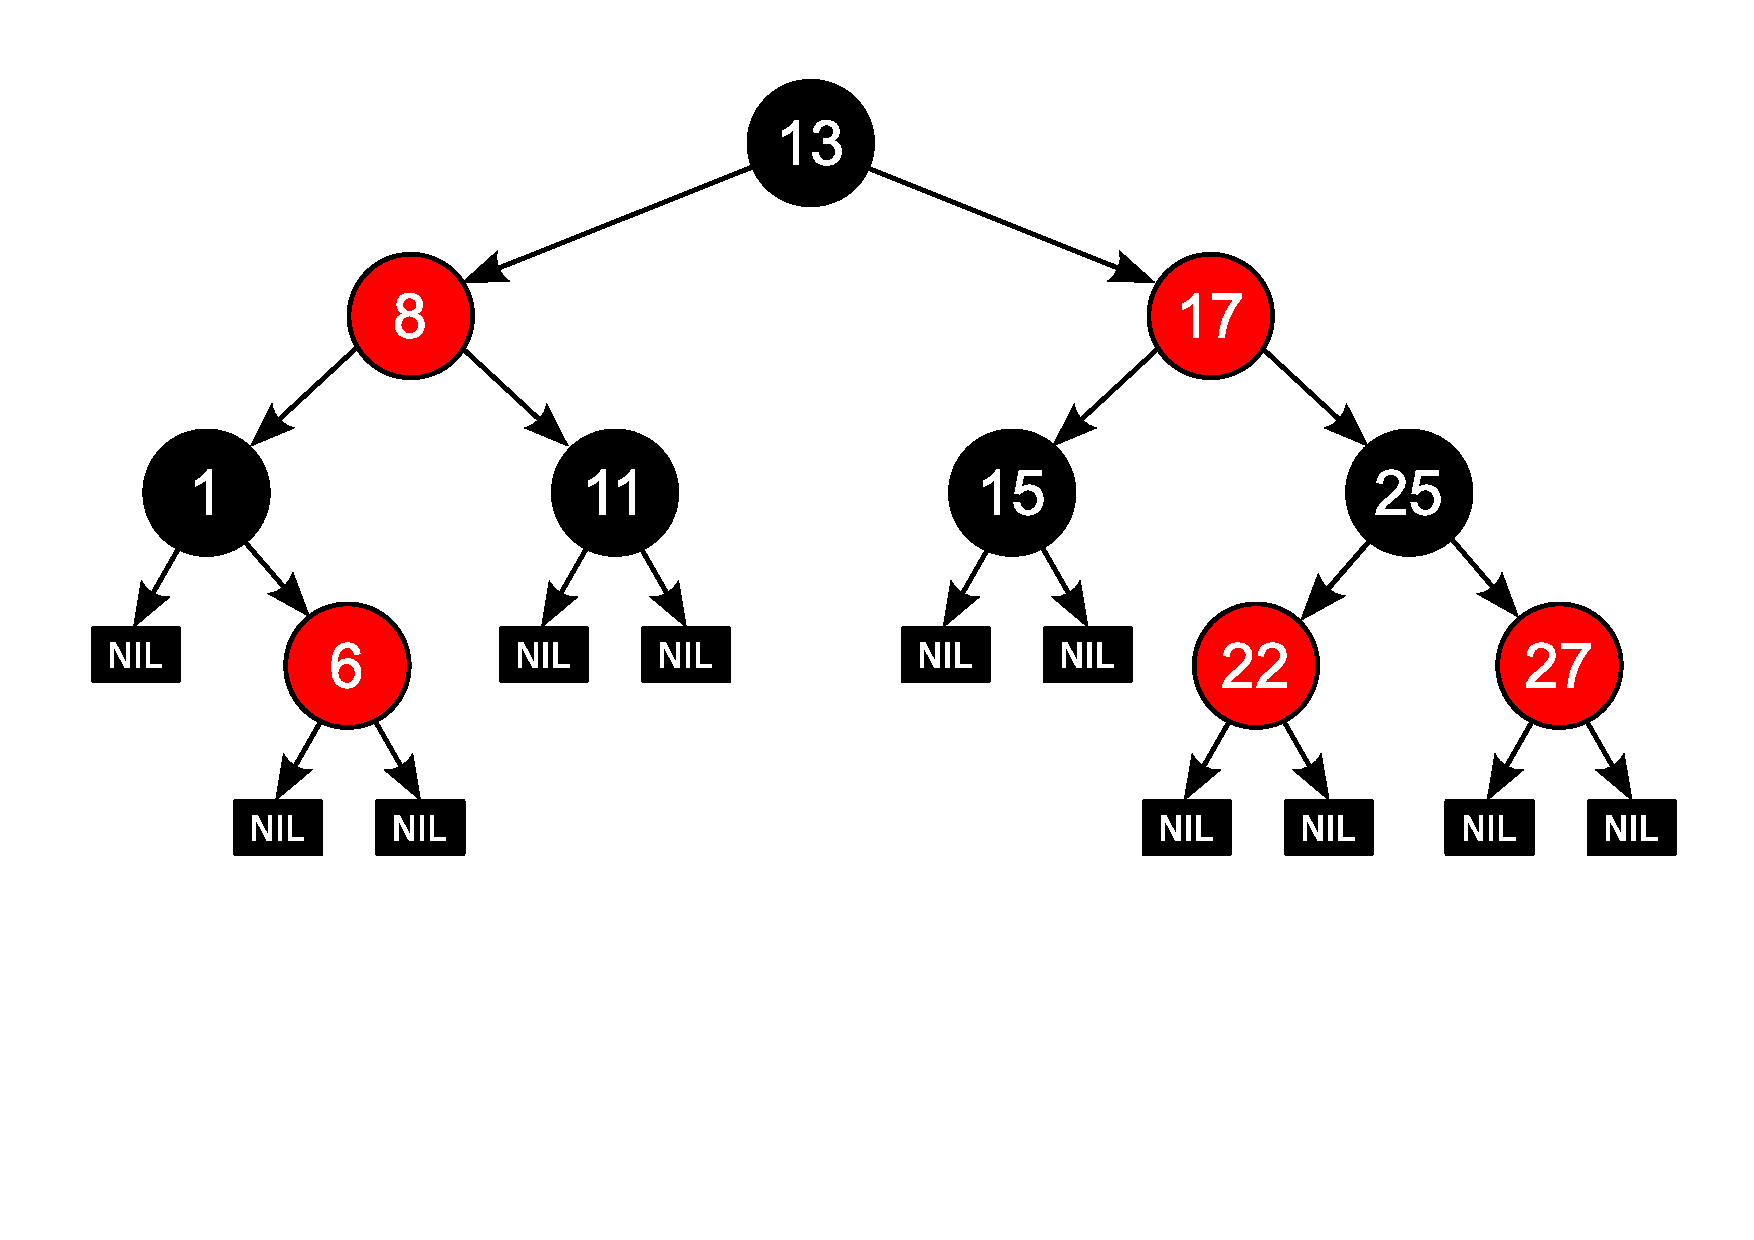
\includegraphics[width=0.479\textwidth]{ADS2/rbtree-example}
    \caption{red-black tree}
\end{figure}


\begin{definition}
    The \hl{black-height} of any node x, denoted by $bh(x)$, is the number of black nodes on any simple path from x (x not included) down to a leaf. bh(Tree)=bh(root). 
\end{definition}

\begin{lemma}
    A red-black tree with $N$ internal nodes has height at most $2\ln (N+1)$. 
\end{lemma}

\subsubsection{Insert}

Insert node as $n$ is red, there exist $n$'s parent $p$, $n$'s uncle $u$, $n$'s grandpa $g$. 
Symmetric is same. 

\begin{enumerate}
    \item Case 1: The tree is empty,  insert the first node.
    \item Case 2: $p$ is root and black, do nothing. 
    \item Case 3: $p$ is root and red, dye $p$ black. 
    \item Case 4
    \begin{enumerate}
        \item Dye $p$ and $u$ nodes black and $g$ node red. 
        \item Recursively maintain $g$ node. 
    \end{enumerate}
    \begin{figure}[H]
        \centering
        \begin{tikzpicture}
            \node (1) at (0,0) [circle, fill=black, text centered, inner sep=0.75pt]{$\textcolor{white}{g}$};
            \node (2) [below left=0.8em of 1] [circle, fill=red, text centered, inner sep=0.75pt]{$\textcolor{white}{p}$};
            \node (3) [below right=0.8em of 1] [circle, fill=red, text centered, inner sep=0.75pt]{$\textcolor{white}{u}$};
            \node (4) [below left=0.8em of 2] [circle, fill=red, text centered, inner sep=0.75pt]{$\textcolor{white}{n}$};
            \node [below=0.2em of 4] {Insert};

            \draw [thick, black, ->] (1)--(2);
            \draw [thick, black, ->] (1)--(3);
            \draw [thick, black, ->] (2)--(4);

            \draw [thick, black, ->] (1.2,-0.5)--(1.8,-0.5);

            \node (1) at (3,0) [circle, fill=red, text centered, inner sep=0.75pt]{$\textcolor{white}{g}$};
            \node (2) [below left=0.8em of 1] [circle, fill=black, text centered, inner sep=0.75pt]{$\textcolor{white}{p}$};
            \node (3) [below right=0.8em of 1] [circle, fill=black, text centered, inner sep=0.75pt]{$\textcolor{white}{u}$};
            \node (4) [below left=0.8em of 2] [circle, fill=red, text centered, inner sep=0.75pt]{$\textcolor{white}{n}$};

            \draw [thick, black, ->] (1)--(3);
            \draw [thick, black, ->] (2)--(4);
            \draw [thick, black, ->] (1)--(2);
        \end{tikzpicture}
    \end{figure}
    
    \item Case 5: Rotate $p$ and then in Case 4. 
    \begin{figure}[H]
        \centering
        \begin{tikzpicture}
            \node (1) at (0,0) [circle, fill=black, text centered, inner sep=0.75pt]{$\textcolor{white}{g}$};
            \node (2) [below left=0.8em of 1] [circle, fill=red, text centered, inner sep=0.75pt]{$\textcolor{white}{p}$};
            \node (3) [below right=0.8em of 1] [circle, fill=black, text centered, inner sep=0.75pt]{$\textcolor{white}{u}$};
            \node (4) [below right=0.8em of 2] [circle, fill=red, text centered, inner sep=0.75pt]{$\textcolor{white}{n}$};
            \node [below=0.2em of 4] {Insert};
            
            \draw [very thick, draw=light_blue, ->] (-0.6,-1.2) arc (-90:180:0.24);

            \draw [thick, black, ->] (1)--(3);
            \draw [thick, black, ->] (2)--(4);
            \draw [thick, black, ->] (1)--(2);

            \draw [thick, black, ->] (1.2,-0.5)--(1.8,-0.5);

            \node (1) at (3,0) [circle, fill=black, text centered, inner sep=0.75pt]{$\textcolor{white}{g}$};
            \node (2) [below left=0.8em of 1] [circle, fill=red, text centered, inner sep=0.75pt]{$\textcolor{white}{n}$};
            \node (3) [below right=0.8em of 1] [circle, fill=black, text centered, inner sep=0.75pt]{$\textcolor{white}{u}$};
            \node (4) [below left=0.8em of 2] [circle, fill=red, text centered, inner sep=0.75pt]{$\textcolor{white}{p}$};

            \draw [thick, black, ->] (1)--(3);
            \draw [thick, black, ->] (2)--(4);
            \draw [thick, black, ->] (1)--(2);
        \end{tikzpicture}
    \end{figure}
    \item Case 6
    \begin{enumerate}
        \item Dye $p$ black and $g$ red. 
        \item Rotate $g$. 
    \end{enumerate}
    \begin{figure}[H]
        \centering
        \begin{tikzpicture}
            \node (1) at (0,0) [circle, fill=black, text centered, inner sep=0.75pt]{$\textcolor{white}{g}$};
            \node (2) [below left=0.8em of 1] [circle, fill=red, text centered, inner sep=0.75pt]{$\textcolor{white}{p}$};
            \node (3) [below right=0.8em of 1] [circle, fill=black, text centered, inner sep=0.75pt]{$\textcolor{white}{u}$};
            \node (4) [below left=0.8em of 2] [circle, fill=red, text centered, inner sep=0.75pt]{$\textcolor{white}{n}$};
            \node [below=0.2em of 4] {Insert};

            \draw [thick, black, ->] (1)--(3);
            \draw [thick, black, ->] (2)--(4);
            \draw [thick, black, ->] (1)--(2);

            \draw [thick, black, ->] (1.2,-0.5)--(1.8,-0.5);

            \node (1) at (3,0) [circle, fill=red, text centered, inner sep=0.75pt]{$\textcolor{white}{g}$};
            \node (2) [below left=0.8em of 1] [circle, fill=black, text centered, inner sep=0.75pt]{$\textcolor{white}{p}$};
            \node (3) [below right=0.8em of 1] [circle, fill=black, text centered, inner sep=0.75pt]{$\textcolor{white}{u}$};
            \node (4) [below left=0.8em of 2] [circle, fill=red, text centered, inner sep=0.75pt]{$\textcolor{white}{n}$};

            \draw [very thick, draw=light_blue, <-] (3.2,-0.8) arc (0:270:0.24);

            \draw [thick, black, ->] (1)--(3);
            \draw [thick, black, ->] (2)--(4);
            \draw [thick, black, ->] (1)--(2);

            \draw [thick, black, ->] (4.2,-0.5)--(4.8,-0.5);

            \node (1) at (6,0) [circle, fill=black, text centered, inner sep=0.75pt]{$\textcolor{white}{p}$};
            \node (2) [below left=0.8em of 1] [circle, fill=red, text centered, inner sep=0.75pt]{$\textcolor{white}{n}$};
            \node (3) [below right=0.8em of 1] [circle, fill=red, text centered, inner sep=0.75pt]{$\textcolor{white}{g}$};
            \node (4) [below right=0.8em of 3] [circle, fill=black, text centered, inner sep=0.75pt]{$\textcolor{white}{u}$};

            \draw [thick, black, ->] (1)--(3);
            \draw [thick, black, ->] (3)--(4);
            \draw [thick, black, ->] (1)--(2);
        \end{tikzpicture}
    \end{figure}
\end{enumerate}



\subsubsection{Delete}
Delete node as $n$ is red, there exist $n$'s parent $p$, $n$'s uncle $u$, $n$'s grandpa $g$, $n$'s son $s$, $n$'s brother $b$, $n$'s nephew $c$ and $e$. 

\textbf{Delete: }
\begin{enumerate}
    \item Case 0: $n$ is root, delete it. 
    \item Case 1: $n$ has degree 2, replace $n$ by the largest one in its left subtree (predecessor), then delete the replacing node from the subtree, after that need to be re-maintained.
    \item Case 2: $n$ has degree 1, replace $n$ by $s$. If $n$ is black, should dye $s$ black. If $s$ is already black, need to be re-maintained. 
    \item Case 3: $n$ is a leaf. If $n$ is red, delete it. Else $n$ is black, delete and then need to be re-maintained. 
\end{enumerate}

\textbf{Re-maintained: }
\begin{enumerate}
    \item Case 1: 
    \begin{enumerate}
        \item Rotate $p$. 
        \item Dye $b$ black and $p$ red. 
        \item Maintain subtree rooted at $p$. 
    \end{enumerate}
    \begin{figure}[H]
        \centering
        \begin{tikzpicture}
            \node (1) at (0,0) [circle, fill=black, text centered, inner sep=0.75pt]{$\textcolor{white}{p}$};
            \node (2) [below left=0.8em of 1] [circle, fill=black, text centered, inner sep=0.75pt]{$\textcolor{white}{n}$};
            \node (3) [below right=0.8em of 1] [circle, fill=red, text centered, inner sep=0.75pt]{$\textcolor{white}{b}$};
            \node (4) [below left=0.8em of 3] [circle, fill=black, text centered, inner sep=0.75pt]{$\textcolor{white}{c}$};
            \node (5) [below right=0.8em of 3] [circle, fill=black, text centered, inner sep=0.75pt]{$\textcolor{white}{e}$};

            \draw [thick, black, ->] (1)--(3);
            \draw [thick, black, ->] (1)--(2);
            \draw [thick, black, ->] (3)--(4);
            \draw [thick, black, ->] (3)--(5);

            \draw [thick, black, ->] (1.2,-0.5)--(1.8,-0.5);

            \node (1) at (3,0) [circle, fill=red, text centered, inner sep=0.75pt]{$\textcolor{white}{b}$};
            \node (2) [below left=0.8em of 1] [circle, fill=black, text centered, inner sep=0.75pt]{$\textcolor{white}{p}$};
            \node (3) [below right=0.8em of 2] [circle, fill=black, text centered, inner sep=0.75pt]{$\textcolor{white}{c}$};
            \node (4) [below left=0.8em of 2] [circle, fill=black, text centered, inner sep=0.75pt]{$\textcolor{white}{n}$};
            \node (5) [below right=0.8em of 1] [circle, fill=black, text centered, inner sep=0.75pt]{$\textcolor{white}{e}$};

            \draw [thick, black, ->] (1)--(5);
            \draw [thick, black, ->] (1)--(2);
            \draw [thick, black, ->] (2)--(4);
            \draw [thick, black, ->] (2)--(3);

            \draw [thick, black, ->] (4.2,-0.5)--(4.8,-0.5);

            \node (1) at (6,0) [circle, fill=black, text centered, inner sep=0.75pt]{$\textcolor{white}{b}$};
            \node (2) [below left=0.8em of 1] [circle, fill=red, text centered, inner sep=0.75pt]{$\textcolor{white}{p}$};
            \node (3) [below right=0.8em of 2] [circle, fill=black, text centered, inner sep=0.75pt]{$\textcolor{white}{c}$};
            \node (4) [below left=0.8em of 2] [circle, fill=black, text centered, inner sep=0.75pt]{$\textcolor{white}{n}$};
            \node (5) [below right=0.8em of 1] [circle, fill=black, text centered, inner sep=0.75pt]{$\textcolor{white}{e}$};

            \draw [thick, black, ->] (1)--(5);
            \draw [thick, black, ->] (1)--(2);
            \draw [thick, black, ->] (2)--(4);
            \draw [thick, black, ->] (2)--(3);
        \end{tikzpicture}
    \end{figure}
    \item Case 2: Dye $b$ red and $p$ black. 
    \begin{figure}[H]
        \centering
        \begin{tikzpicture}
            \node (1) at (0,0) [circle, fill=red, text centered, inner sep=0.75pt]{$\textcolor{white}{p}$};
            \node (2) [below left=0.8em of 1] [circle, fill=black, text centered, inner sep=0.75pt]{$\textcolor{white}{n}$};
            \node (3) [below right=0.8em of 1] [circle, fill=black, text centered, inner sep=0.75pt]{$\textcolor{white}{b}$};
            \node (4) [below left=0.8em of 3] [circle, fill=black, text centered, inner sep=0.75pt]{$\textcolor{white}{c}$};
            \node (5) [below right=0.8em of 3] [circle, fill=black, text centered, inner sep=0.75pt]{$\textcolor{white}{e}$};

            \draw [thick, black, ->] (1)--(3);
            \draw [thick, black, ->] (1)--(2);
            \draw [thick, black, ->] (3)--(4);
            \draw [thick, black, ->] (3)--(5);

            \draw [thick, black, ->] (1.2,-0.5)--(1.8,-0.5);

            \node (1) at (3,0) [circle, fill=black, text centered, inner sep=0.75pt]{$\textcolor{white}{p}$};
            \node (2) [below left=0.8em of 1] [circle, fill=black, text centered, inner sep=0.75pt]{$\textcolor{white}{n}$};
            \node (3) [below right=0.8em of 1] [circle, fill=red, text centered, inner sep=0.75pt]{$\textcolor{white}{b}$};
            \node (4) [below left=0.8em of 3] [circle, fill=black, text centered, inner sep=0.75pt]{$\textcolor{white}{c}$};
            \node (5) [below right=0.8em of 3] [circle, fill=black, text centered, inner sep=0.75pt]{$\textcolor{white}{e}$};

            \draw [thick, black, ->] (1)--(3);
            \draw [thick, black, ->] (1)--(2);
            \draw [thick, black, ->] (3)--(4);
            \draw [thick, black, ->] (3)--(5);

            \draw [thick, black, ->] (4.2,-0.5)--(4.8,-0.5);

            \node (1) at (5.4,0) [circle, fill=black, text centered, inner sep=0.75pt]{$\textcolor{white}{p}$};
            % \node (2) [below left=0.8em of 1] [circle, fill=black, text centered, inner sep=0.75pt]{$\textcolor{white}{n}$};
            \node (3) [below right=0.8em of 1] [circle, fill=red, text centered, inner sep=0.75pt]{$\textcolor{white}{b}$};
            \node (4) [below left=0.8em of 3] [circle, fill=black, text centered, inner sep=0.75pt]{$\textcolor{white}{c}$};
            \node (5) [below right=0.8em of 3] [circle, fill=black, text centered, inner sep=0.75pt]{$\textcolor{white}{e}$};

            \draw [thick, black, ->] (1)--(3);
            % \draw [thick, black, ->] (1)--(2);
            \draw [thick, black, ->] (3)--(4);
            \draw [thick, black, ->] (3)--(5);
        \end{tikzpicture}
    \end{figure}
    \item Case 3: Dye $b$ black, recursively maintain $p$. 
    \begin{figure}[H]
        \centering
        \begin{tikzpicture}
            \node (1) at (0,0) [circle, fill=black, text centered, inner sep=0.75pt]{$\textcolor{white}{p}$};
            \node (2) [below left=0.8em of 1] [circle, fill=black, text centered, inner sep=0.75pt]{$\textcolor{white}{n}$};
            \node (3) [below right=0.8em of 1] [circle, fill=black, text centered, inner sep=0.75pt]{$\textcolor{white}{b}$};
            \node (4) [below left=0.8em of 3] [circle, fill=black, text centered, inner sep=0.75pt]{$\textcolor{white}{c}$};
            \node (5) [below right=0.8em of 3] [circle, fill=black, text centered, inner sep=0.75pt]{$\textcolor{white}{e}$};

            \draw [thick, black, ->] (1)--(3);
            \draw [thick, black, ->] (1)--(2);
            \draw [thick, black, ->] (3)--(4);
            \draw [thick, black, ->] (3)--(5);

            \draw [thick, black, ->] (1.2,-0.5)--(1.8,-0.5);

            \node (1) at (3,0) [circle, fill=black, text centered, inner sep=0.75pt]{$\textcolor{white}{p}$};
            \node (2) [below left=0.8em of 1] [circle, fill=black, text centered, inner sep=0.75pt]{$\textcolor{white}{n}$};
            \node (3) [below right=0.8em of 1] [circle, fill=red, text centered, inner sep=0.75pt]{$\textcolor{white}{b}$};
            \node (4) [below left=0.8em of 3] [circle, fill=black, text centered, inner sep=0.75pt]{$\textcolor{white}{c}$};
            \node (5) [below right=0.8em of 3] [circle, fill=black, text centered, inner sep=0.75pt]{$\textcolor{white}{e}$};

            \draw [thick, black, ->] (1)--(3);
            \draw [thick, black, ->] (1)--(2);
            \draw [thick, black, ->] (3)--(4);
            \draw [thick, black, ->] (3)--(5);
        \end{tikzpicture}
    \end{figure}
    \item Case 4: 
    \begin{enumerate}
        \item Rotate $b$. 
        \item Dye $c$ red, $b$ black. 
        \item Then in Case 5. 
    \end{enumerate}
    \begin{figure}[H]
        \centering
        \begin{tikzpicture}
            \node (1) at (0,0) [circle, draw=black, text centered, inner sep=0.75pt]{$\textcolor{black}{p}$};
            \node (2) [below left=0.8em of 1] [circle, fill=black, text centered, inner sep=0.75pt]{$\textcolor{white}{n}$};
            \node (3) [below right=0.8em of 1] [circle, fill=black, text centered, inner sep=0.75pt]{$\textcolor{white}{b}$};
            \node (4) [below left=0.8em of 3] [circle, fill=red, text centered, inner sep=0.75pt]{$\textcolor{white}{c}$};
            \node (5) [below right=0.8em of 3] [circle, fill=black, text centered, inner sep=0.75pt]{$\textcolor{white}{e}$};

            \draw [thick, black, ->] (1)--(3);
            \draw [thick, black, ->] (1)--(2);
            \draw [thick, black, ->] (3)--(4);
            \draw [thick, black, ->] (3)--(5);

            \draw [thick, black, ->] (1.2,-0.5)--(1.8,-0.5);

            \node (1) at (3,0) [circle, draw=black, text centered, inner sep=0.75pt]{$\textcolor{black}{p}$};
            \node (2) [below left=0.8em of 1] [circle, fill=black, text centered, inner sep=0.75pt]{$\textcolor{white}{n}$};
            \node (3) [below right=0.8em of 1] [circle, fill=red, text centered, inner sep=0.75pt]{$\textcolor{white}{c}$};
            \node (4) [below right=0.8em of 3] [circle, fill=black, text centered, inner sep=0.75pt]{$\textcolor{white}{b}$};
            \node (5) [below right=0.8em of 4] [circle, fill=black, text centered, inner sep=0.75pt]{$\textcolor{white}{e}$};

            \draw [thick, black, ->] (1)--(3);
            \draw [thick, black, ->] (1)--(2);
            \draw [thick, black, ->] (3)--(4);
            \draw [thick, black, ->] (4)--(5);

            \draw [thick, black, ->] (4.2,-0.5)--(4.8,-0.5);

            \node (1) at (6,0) [circle, draw=black, text centered, inner sep=0.75pt]{$\textcolor{black}{p}$};
            \node (2) [below left=0.8em of 1] [circle, fill=black, text centered, inner sep=0.75pt]{$\textcolor{white}{n}$};
            \node (3) [below right=0.8em of 1] [circle, fill=black, text centered, inner sep=0.75pt]{$\textcolor{white}{c}$};
            \node (4) [below right=0.8em of 3] [circle, fill=red, text centered, inner sep=0.75pt]{$\textcolor{white}{b}$};
            \node (5) [below right=0.8em of 4] [circle, fill=black, text centered, inner sep=0.75pt]{$\textcolor{white}{e}$};

            \draw [thick, black, ->] (1)--(3);
            \draw [thick, black, ->] (1)--(2);
            \draw [thick, black, ->] (3)--(4);
            \draw [thick, black, ->] (4)--(5);
        \end{tikzpicture}
    \end{figure}
    \item Case 5:
    \begin{enumerate}
        \item Rotate $p$. 
        \item Swap the color of $p$ and $b$. 
        \item Dye distant nephew $e$ black. 
    \end{enumerate}
    \begin{figure}[H]
        \centering
        \begin{tikzpicture}
            \node (1) at (0,0) [circle, draw=black, text centered, inner sep=0.75pt]{$\textcolor{black}{p}$};
            \node (2) [below left=0.8em of 1] [circle, fill=black, text centered, inner sep=0.75pt]{$\textcolor{white}{n}$};
            \node (3) [below right=0.8em of 1] [circle, fill=black, text centered, inner sep=0.75pt]{$\textcolor{white}{b}$};
            \node (4) [below right=0.8em of 3] [circle, fill=red, text centered, inner sep=0.75pt]{$\textcolor{white}{e}$};

            \draw [thick, black, ->] (1)--(3);
            \draw [thick, black, ->] (1)--(2);
            \draw [thick, black, ->] (3)--(4);

            \draw [thick, black, ->] (1.2,-0.5)--(1.8,-0.5);

            \node (1) at (3,0) [circle, fill=black, text centered, inner sep=0.75pt]{$\textcolor{white}{b}$};
            \node (2) [below left=0.8em of 1] [circle, draw=black, text centered, inner sep=0.75pt]{$\textcolor{black}{p}$};
            \node (3) [below left=0.8em of 2] [circle, fill=black, text centered, inner sep=0.75pt]{$\textcolor{white}{n}$};
            \node (4) [below right=0.8em of 1] [circle, fill=red, text centered, inner sep=0.75pt]{$\textcolor{white}{e}$};

            \draw [thick, black, ->] (1)--(2);
            \draw [thick, black, ->] (1)--(4);
            \draw [thick, black, ->] (2)--(3);

            \draw [thick, black, ->] (4.2,-0.5)--(4.8,-0.5);

            \node (1) at (6,0) [circle, draw=black, text centered, inner sep=0.75pt]{$\textcolor{black}{b}$};
            \node (2) [below left=0.8em of 1] [circle, fill=black, text centered, inner sep=0.75pt]{$\textcolor{white}{p}$};
            \node (3) [below left=0.8em of 2] [circle, fill=black, text centered, inner sep=0.75pt]{$\textcolor{white}{n}$};
            \node (4) [below right=0.8em of 1] [circle, fill=black, text centered, inner sep=0.75pt]{$\textcolor{white}{e}$};

            \draw [thick, black, ->] (1)--(2);
            \draw [thick, black, ->] (1)--(4);
            \draw [thick, black, ->] (2)--(3);

            \draw [thick, black, ->] (6,-1)--(6,-1.6);

            \node (1) at (6,-2) [circle, draw=black, text centered, inner sep=0.75pt]{$\textcolor{black}{b}$};
            \node (2) [below left=0.8em of 1] [circle, fill=black, text centered, inner sep=0.75pt]{$\textcolor{white}{p}$};
            % \node (3) [below left=0.8em of 2] [circle, fill=black, text centered, inner sep=0.75pt]{$\textcolor{white}{n}$};
            \node (4) [below right=0.8em of 1] [circle, fill=black, text centered, inner sep=0.75pt]{$\textcolor{white}{e}$};

            \draw [thick, black, ->] (1)--(2);
            \draw [thick, black, ->] (1)--(4);
            % \draw [thick, black, ->] (2)--(3);
        \end{tikzpicture}
    \end{figure}
\end{enumerate}

\subsubsection{Relationship between red-black tree and 4-order B-tree (2-3-4 tree)}

We can even say that the red-black tree and the 4-order B-tree (2-3-4 tree) are equivalent in structure.

\begin{figure}[H]
    \centering
    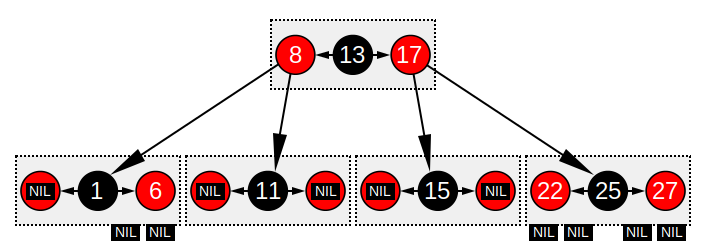
\includegraphics[width=0.479\textwidth]{ADS2/rbtree-btree-analogy}
    \caption{rbtree-btree-analogy}
\end{figure}


\subsection{B+ Trees}
\begin{definition}
    A \hl{B+ tree} of order (阶) \hl{$M$} is a tree with the following structural properties: 
    \begin{enumerate}
        \item The root is either a leaf or has \hl{between 2 and M children}. 
        \item All nonleaf nodes (except the root) have \hl{between $\left \lceil \frac{M}{2} \right \rceil $ and $M$ children}. 
        \item All leaves are at the \hl{same depth}. 
    \end{enumerate}
\end{definition}

\begin{figure}[H]
    \centering
    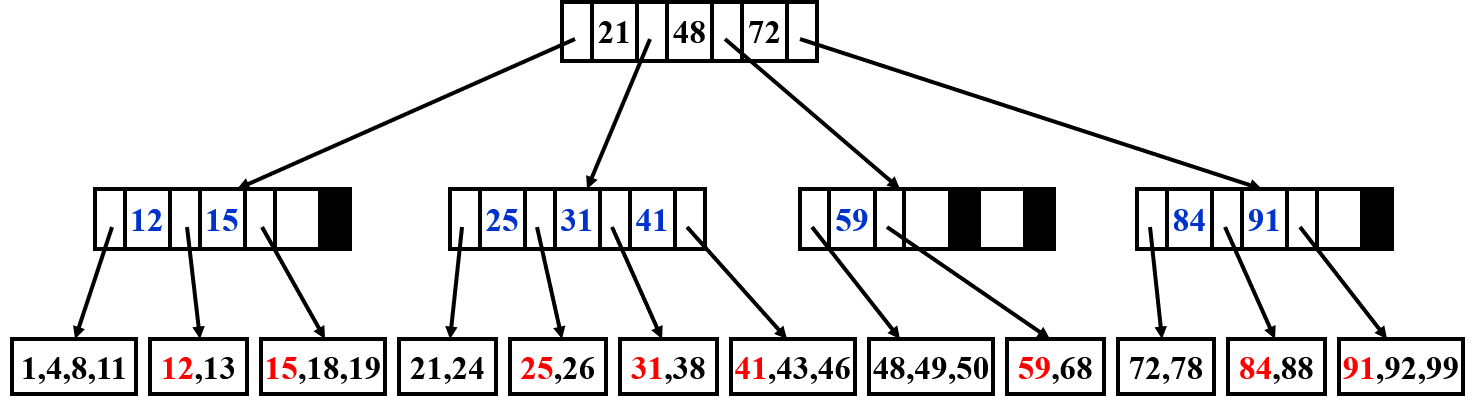
\includegraphics[width=0.479\textwidth]{ADS2/A B+ tree of order 4}
    \caption{A B+ tree of order 4 (2-3-4 tree)}
\end{figure}

\begin{enumerate}
    \item find
    \item insert
    \item delete
\end{enumerate}

$Depth(M,N)=O(\left \lceil \log_{\left \lceil  \frac{M}{2} \right \rceil} N \right \rceil)$